\documentclass[a4paper,11pt]{article}
\usepackage[margin=25mm]{geometry}
\usepackage[T1]{fontenc}
\usepackage[utf8]{inputenc}
\usepackage{amsmath,amssymb,graphicx,booktabs,array}
\usepackage{microtype,placeins,setspace}
\onehalfspacing
\pagestyle{plain}
\usepackage[font=small,labelfont=bf]{caption}
\usepackage[colorlinks=true,allcolors=blue,pdfauthor={}]{hyperref}
\newcommand{\gtd}{\ensuremath{\gamma\!\rightarrow\!\delta}}
\newcommand{\dtg}{\ensuremath{\delta\!\rightarrow\!\gamma}}
\title{Additional file 1: supplementary methods and sensitivity analyses}
\author{}
\date{}
\renewcommand{\thefigure}{S\arabic{figure}}
\renewcommand{\thetable}{S\arabic{table}}
\renewcommand{\thesection}{S\arabic{section}}
\begin{document}
\maketitle
\section{Pretraining pools and data provenance}
Single-chain inputs total 194887 gamma and 1262692 delta sequences before
pretraining filters. All chains appearing in the paired corpus are excluded
from pretraining, and sequences shorter than six residues are removed. The main
pretraining training pool contains 187092 gamma and 1230589 delta sequences,
with validation sets of 3818 and 25114 sequences. Training and validation are
fully disjoint at the unique CDR3-sequence level. Source experiments
use an additional study-excluded pool containing 186949 gamma and 1230167
delta training sequences, with 3815 and 25106 validation sequences. Both source
protocols use the same filtered pretraining pool. SHA256 manifests identify raw, processed, split and provenance artifacts;
training seeds, selected-checkpoint identifiers and actual exposure appear in Additional file 3.


\section{Corruption and reconstruction}
Each single-chain sequence is assigned a masking rate of 15\% or 30\% with equal
probability. Exactly the larger of one and the rounded rate times sequence
length is selected without replacement. Each selected residue independently
receives a mask token (80\%), a uniform canonical amino acid (10\%) or its
original token (10\%). Deletion starts are sampled uniformly, with span lengths
uniformly 1--3, until at least the rounded 8\% target is covered; spans can
overshoot that target. Deletion follows masking and can overlap selected sites.
The damaged mask includes selected-but-unchanged residues and deleted sites.
The aligned-copy control copies the corrupted aligned token and uses a mask at
deleted sites. Reconstruction includes EOS in token NLL; residue accuracy is
separately evaluated on original residue positions. No reconstruction metric
is interpreted as partner recovery.


\subsection{Denoising pretraining improves single-chain reconstruction}
On the frozen square-root-pretrained validation corruptions, selected-residue
accuracy is 71.3\% and 70.3\% for gamma and 64.1\% and 64.7\% for delta across
the two seeds. Corresponding aligned-copy accuracy is 6.9\%/6.3\% for gamma and
6.7\%/6.2\% for delta. This shows reconstruction beyond the specified aligned-copy sanity control. It does not establish that pretraining improves recorded partner
recovery; that question requires the downstream matched comparisons.


\section{Generator training and matched controls}
The generator is a shared encoder--decoder Transformer with 7396890 parameters,
four encoder and four decoder layers, width 256, eight attention heads,
feedforward width 1024 and dropout 0.1. It tokenizes individual amino acids with
chain identity and control tokens, using a maximum of 64 tokens. The two
conditionals share parameters:
\begin{equation}
p_\theta(d\mid g),\qquad p_\theta(g\mid d).
\end{equation}
Training minimizes teacher-forced target-token negative log likelihood (NLL),
including the end-of-sequence (EOS) token and excluding the chain-control
prediction from the loss.

Denoising uses 20000 steps, batch size 1024, AdamW at learning rate
$3\times10^{-4}$ and 500 warmup steps. Each sequence is masked at 15\% or 30\%
with equal probability. Selected residues are replaced by mask/random/unchanged
tokens at 80/10/10 proportions, followed by short-span deletions targeting
approximately 8\% of positions. Reconstruction is evaluated separately on
corruption-selected residues and against an aligned copy control. The saved
``damaged'' mask includes selected-but-unchanged positions in the 80/10/10 rule
as well as deleted positions; it is not restricted to visibly altered residues.
These teacher-forced
metrics are not free partner-generation accuracy. Raw-frequency, square-root,
balanced, gamma-only and delta-only chain mixtures use the same total number of
sequence draws. Sequence and target-token exposure are reported separately.
The square-root checkpoints are reused from the pair-excluded historical
pretraining, with independently evaluated frozen corruption.

Paired fine-tuning uses at most 1500 steps at batch size 256, learning rate
$2\times10^{-5}$, 200 warmup steps, validation every 100 steps and patience five.
The selection criterion averages known-partner NLL within query, then queries
within direction. Bidirectional models average the two directions equally;
directional exposure diagnostics select using their specified direction only.
Sampling chooses modeled directions equally, input queries uniformly and one
recorded partner uniformly per query.
The constant-source control changes only source residues while retaining
initialization, target sampling and optimization. Random initialization changes only initial weights. It matches downstream
training settings but receives no denoising pretraining, so this is not a
matched-total-computation comparison. Shuffled-input evaluation applies a
deterministic query permutation to the fitted conditional model, disrupting the
input--recorded-partner association. Edge-uniform sampling is a separate control.
Table~\ref{tab:controls} summarizes the roles of these four controls.

The unidirectional sensitivity controls receive at most 750 steps and 100
warmup steps, matching nominal per-direction sequence exposure. Directional
exposure diagnostics instead retain the 1500-step maximum. Actual exposure under early
stopping is recorded. Data-efficiency comparisons use nested complete-component
subsets and both pretrained and random models. The 10/25/50/100\% labels
correspond to 725/1814/2249/7254 edges. The nominal 50\% subset is only 31.0\%
because the 5005-edge component cannot be split. The curve therefore changes
component composition as well as sample size.
All three smaller subsets consist exclusively of singleton components.

The conditional and constant-source generators share initialization, target
sampling, optimizer and nominal downstream budget. Constant-source input keeps
the chain token and removes source residues. Random initialization removes
pretraining and retains downstream settings; total training computation is not
matched. Shuffled-input evaluation permutes queries without fixed points and
keeps the original recorded-partner labels. A separate copy of the fine-tuned
generator initializes the ranker. Its copied encoder is trainable; the source
generator is not updated. All paired fits use the same protocol-specific
training edges. Seeds, selected checkpoints and actual exposure accompany
Additional file 3.

AdamW uses weight decay 0.01 and gradient-norm clipping at 1.0. For denoising and
generator training, the per-step learning rate is the nominal rate multiplied
by $\min(1,s/w)$ and $[1+\cos(\pi\min(1,s/S))]/2$, where $s$ is the current
step, $w$ the warmup and $S$ the nominal maximum steps. This applies cosine
decay over the whole nominal run, including warmup. Ranker training uses its
fixed stated learning rate. Training may stop early; actual exposures, not only
nominal limits, are retained.


\begin{table}[htbp]
\centering
\caption{Core generator controls. All conditions retain the protocol-specific test query population and fixed primary sampling rule.}
\label{tab:controls}
\begin{tabular}{p{0.30\linewidth}p{0.64\linewidth}}
\toprule
Condition & Comparison purpose\\
\midrule
Pretrained conditional & Uses the input chain after denoising pretraining.\\
Constant-source target prior & Removes source residues while matching initialization, target sampling and downstream optimization.\\
Random initialization & Removes denoising pretraining; the downstream budget is matched, total computation is not.\\
Shuffled input & Breaks the input--recorded-partner association at evaluation using the fitted conditional model.\\
\bottomrule
\end{tabular}
\end{table}


\section{Secondary ranker and reference scorers}
The pair ranker evaluates whether an additional scoring stage helps order the
generator's candidates; it is a secondary evaluation component.
The ranker starts from a separate copy of the selected condition-specific
generator's encoder, after paired fine-tuning. It uses amino-acid-only pooling,
128-dimensional chain-specific projections, a normalized vector dot product
and a two-layer interaction head with hidden width 256 and dropout 0.15 over
the concatenated vectors, their product and absolute difference. The copied encoder and ranking head are optimized on the same training edges
used by the generator. The original generator remains frozen, but the copied
encoder is trainable. Separate training refers to the subsequent parameters
and optimization; neither the representations nor the cohort are independent. Training uses 3000 steps
at batch size 256 and learning rate $3\times10^{-4}$. The first 1500 steps use
multi-positive contrastive loss; the remaining steps use constructed-negative
binary cross-entropy (BCE). The primary negative ratio is three per positive, with
half random and half length/terminal-motif matched draws. Ratios one and five
and random-only training provide sensitivity controls. All negative construction
uses training edges only; known training partners are excluded. The best mean
directional selection-validation MRR after explicit-negative training begins
selects the checkpoint.
Positive and constructed-negative classes receive equal BCE loss weight at
every ratio; increasing the ratio changes negative sampling diversity rather
than the total weight of the negative class.

Fixed-pool scorers include conditional likelihood, target-prior likelihood,
deterministically shuffled-input likelihood, their conditional-minus-prior
likelihood difference, ranker, fused score and seeded random scores.
Likelihood scores are negative per-target-token NLL, including EOS; thus the
likelihood difference uses length-normalized log scores rather than the raw
sequence log-probability ratio. Additional
controls are training-target frequency, a shallow length/terminal-feature
logistic model and an exact two-chain edit-neighbor score. For a candidate
$(g,d)$ and training edge set $E_{\rm tr}$, the latter is
\begin{equation}
s_{\rm NN}(g,d)=-\min_{(g',d')\in E_{\rm tr}}
\frac{1}{2}\left[
\frac{\operatorname{Lev}(g,g')}{\max(|g|,|g'|)}+
\frac{\operatorname{Lev}(d,d')}{\max(|d|,|d'|)}\right].
\end{equation}
Every training edge contributes to the minimum. The shallow control is fitted
to training positives and mixed constructed negatives at ratio 1:3, selecting
$C\in\{0.1,1,10\}$ by mean Hit@5 across the four small selection-validation pools.

A complementary nearest-input partner-transfer baseline finds the closest
training input using normalized full-CDR3 Levenshtein distance, resolves ties
lexicographically, and proposes that input's recorded training partners. Targets
are ordered by descending training degree and then lexicographically, retaining
at most 64 unique candidates. A fixed five-neighbor sensitivity concatenates
those lists in neighbor order. No test target is injected into these proposals;
under exact target exclusion their recovery is necessarily zero. For frozen
retrieval pools, a separate nearest-input partner-similarity score ranks each
candidate by its minimum normalized distance to any partner of the single
nearest training input. This similarity extension scores truth-containing
pools and is not direct partner transfer.


\section{Candidate construction and score calibration}
The primary ranker first uses multi-positive contrastive training, then equally
weighted positive and constructed-negative binary cross-entropy. Three negative
draws per positive are drawn from supervised-training combinations, excluding
known training partners. The mixed policy combines random and length/terminal
matching; actual fallbacks and draw counts are recorded. Unrecorded combinations
are not biological negatives. Sensitivities change ratios to one or five, or
use random-only draws. Fixed retrieval pools inject all role-specific recorded
positives and up to 100 unrecorded targets from that role's universe. Other
recorded partners are excluded from distractors. Random, length, terminal-motif
and normalized-edit matching are deterministic at fixed seed. All scorers use
the same frozen lists. Free sampling instead makes 64 draws with temperature
one and top-p 0.95; 6--35 canonical residues and observed EOS are required.
Invalid and duplicate draws are never replaced. Training-target exclusion is
an explicitly separate policy that can delete legitimate exposed positives.

For each negative draw, the source direction is chosen with equal probability.
Under the mixed policy, a hard draw is chosen with probability 0.5. Candidate
training targets within one residue of the reference target length are sorted
by absolute length difference, mismatch count over the first and last three
residues, then sequence. The draw is uniform over the first 64 eligible targets
after known-training-partner exclusion. If none remain, sampling falls back to
uniform random eligible training targets. Sampling is with replacement;
no held-out pairing labels filter training negatives. The two BCE classes each
receive one-half of the loss weight at every negative ratio.

Fixed-pool length matching sorts eligible role targets by the minimum length
gap to a role-specific positive, then normalized full-CDR3 edit distance and
sequence. Motif matching uses the sum of Levenshtein distances over the first
and last three residues, then full normalized edit distance and sequence. Edit
matching uses full normalized distance and sequence. Random pools sample
without replacement. Candidate targets are lexicographically stored, and score
ties use that order. Truth-containing retrieval is an explicitly constructed
diagnostic; no such positive-directed pool construction is used in free sampling.


The primary setting uses 64 draws at temperature one and top-$p=0.95$.
Split-17 primary conditional and constant-source models save 256 draws and
reuse prefixes of 16, 64 and 256. A prespecified six-cell temperature/top-$p$
grid is inspected on split-17 tuning data but does not replace the primary
setting. Validity requires 6--35 canonical residues and an observed EOS token,
allowing 36 decoding steps. Invalid or duplicate draws are not replaced.
Candidates are evaluated both with and without exact training targets. The
exclusion policy may remove legitimate recorded positives in exposed-target
settings, and is reported only as a separate sensitivity analysis. Free
generation does not guarantee that any recorded partner exists among candidates.

For each split and query, fixed candidate pools contain all role-specific
recorded positives and up to 100 unrecorded targets sampled from that split's
target universe using random, length, terminal-motif or edit-neighbor matching.
Full-target retrieval uses the same universe. Other recorded partners are
excluded from distractors without being added as role-specific test positives.
All scorers and model seeds share frozen candidate lists. Unlike free generation,
these retrieval pools include the true targets by construction.
Score ties are resolved by lexicographic target-sequence order. In the primary
chain-disjoint tests, every training-frequency score is zero, so that baseline
is a deterministic tie-order control, not informative frequency prediction.

Direction-specific score means and population standard deviations are estimated
on tuning candidates. A ranker fusion weight from $\{0,.25,.5,.75,1\}$ is shared
across directions and selected by direction-balanced query-macro Hit@5, with
ties favoring less ranker weight. Free and fixed-pool calibration are separate.
An independent calibration subset selects the acceptance threshold by balanced
accuracy against recorded positives and constructed unrecorded combinations;
ties favor the highest threshold, including reject-all. No-positive or
no-negative calibration yields reject-all. Acceptance curves apply fixed
calibration-score quantiles and both endpoints to test data. Pooled AUROC and
AUPRC are reported with positive prevalence, consistent with the limitations of
imbalanced classification summaries (see the precision--recall reference in the main manuscript). These labels and scores
do not define biological specificity or binding probability.


\section{Metric definitions, uncertainty and distance strata}
For query $q$, let $P_q$ be its recorded test partners, $C_q$ its unique valid
candidates and $C_q^{(K)}$ its first $K$ ranked candidates. Define
\begin{equation}
\mathrm{Coverage}(q)=\mathbf{1}(P_q\cap C_q\ne\varnothing),\qquad
H_K(q)=\mathbf{1}(P_q\cap C_q^{(K)}\ne\varnothing).
\end{equation}
\begin{equation}
R_K(q)=\frac{|P_q\cap C_q^{(K)}|}{|P_q|}.
\end{equation}
If $r_q(t)$ is the one-based candidate rank, reciprocal rank is
$1/\min_{t\in P_q\cap C_q}r_q(t)$ when a partner is present and zero otherwise.
Mean positive rank is $|P_q|^{-1}\sum_{t\in P_q}\widetilde r_q(t)$,
where $\widetilde r_q(t)=r_q(t)$ for present partners and $|C_q|+1$ for absent
partners. MRR averages reciprocal rank across queries. We report query-macro outcomes and positive-count-weighted query
outcomes; the latter yields edge-micro Recall. The primary endpoint is the
equal-direction mean of query-macro Hit@5 at 64 draws, reported separately for
likelihood, ranker and fused ordering. Per-fit event counts and query-level results appear in Additional file 4;
all frozen retrieval pools, candidate hashes and split assignments are supplied
in Additional file 5. Ranker and fused ordering assess the same generator
candidates and do not constitute additional generation methods.
NLL, token-weighted NLL, raw ordering,
validity, uniqueness, novelty and diversity are secondary summaries.

The reported query-macro NLL first averages the target-token losses for each
recorded partner, including EOS and excluding padding and the chain-control
prediction. For target sequence $y$, let $T_y=|y|+1$, with EOS at position $T_y$.
For the query set $Q_d$ in direction $d$, the implemented hierarchy is
\begin{align}
\ell(q,y)&=-\frac{1}{T_y}\sum_{i=1}^{T_y}
 \log p_\theta(y_i\mid q,y_{<i}),\\
L_d&=\frac{1}{|Q_d|}\sum_{q\in Q_d}
 \frac{1}{|P_q|}\sum_{y\in P_q}\ell(q,y),\qquad
L_{\rm macro}=\frac{L_{\gamma\rightarrow\delta}
 +L_{\delta\rightarrow\gamma}}{2}.
\end{align}
Thus, partners within a query and queries within a direction receive equal
weight; longer targets do not receive more weight in this summary.
Checkpoint selection uses this same hierarchy on the selection partition
(one direction only for directional fits).
The separately reported token-weighted NLL instead divides the sum of all
recorded target-token losses by their total token count within each direction.
The optimization loss also averages non-ignored target tokens within each
training minibatch; it is distinct from the query-macro reporting hierarchy.

We use 2000 paired cluster-bootstrap replicates over complete test components,
or source-query groups for directional tasks. Joint directional endpoints use
the same component resample but average direction-specific query means equally.
Model comparisons align query identities, positives and cluster labels; fixed
pools must also have identical hashes. Two model seeds are averaged within each
split before the descriptive mean and sample standard deviation across the
three split means are calculated. These SDs are not confidence intervals.
Repeated splits and seeds are not independent biological subjects. Intervals
condition on fitted models and saved candidates, and are descriptive without
family-wise multiplicity adjustment. Zero-event percentile intervals of $[0,0]$
are not population upper bounds; an explicitly labeled iid Wilson reference is
provided for binary query events only, not fractional Recall.

Every paired chain is compared with supervised and pretraining references using
raw and length-normalized Levenshtein distances on complete CDR3, internal
residues (excluding three residues at each end) and terminal residues. Exact
minimum witnesses are saved. Full-sequence strata are 0, 1, 2 and at least 3.
The distant subset requires both source and eligible recorded target to be at
distance at least three from both reference pools. Edge-defined strata retain
the original candidate lists and test-cluster identities. Empty and single-cluster
strata are explicit. Source, length, number of partners and training-target
overlap are additional descriptive strata.


\section{Pretraining and negative-sampling sensitivity}
\subsection{Pretraining mixture and downstream sampling have distinct effects}
The two-seed downstream NLL means for square-root, raw and balanced pretraining
are, respectively, 1.256/0.754, 1.255/0.757 and 1.259/0.755 for \gtd{}/\dtg{}
on split 17 (Figure~\ref{fig:figure_S1_pretraining}). Raw-minus-square-root
equal-direction differences are approximately 0.001 nats per token in both
fits, with paired intervals crossing zero. Balanced-minus-square-root
differences are approximately 0.002 in both fits, with intervals above zero.
These small NLL differences do not select a new primary mixture after testing.

Restricting pretraining to one chain has larger directional effects. Gamma-only
initialization gives downstream NLL 1.294/0.755, while delta-only initialization
gives 1.257/0.779. On frozen denoising validation, gamma-only pretraining yields
39.6\% selected-site accuracy for delta, and delta-only pretraining yields
27.3\% for gamma, compared with 64.4\% and 70.8\% under the square-root
mixture. The results are consistent with chain-specific reconstruction exposure
affecting the target-sequence prior. Equal total sequence draws do not equate
chain-specific or token exposure, and these teacher-forced differences do not
demonstrate reliable free partner recovery.

Edge-uniform paired training gives NLL 1.263/0.759, compared with 1.256/0.754
under query-uniform training. Its equal-direction excess is approximately
0.006 nats per token in both fitted seeds, with paired intervals above zero.
The nominally direction-budget-matched unidirectional models give NLL
1.258 for \gtd{} and 0.756 for \dtg{}, close to the bidirectional model.
All these settings retain sparse free-recovery events. Their actual early-stop
and token exposure records accompany the matched nominal budgets; the comparison
does not establish a universal benefit from sharing the two directions.

\begin{figure}[!htbp]
\centering
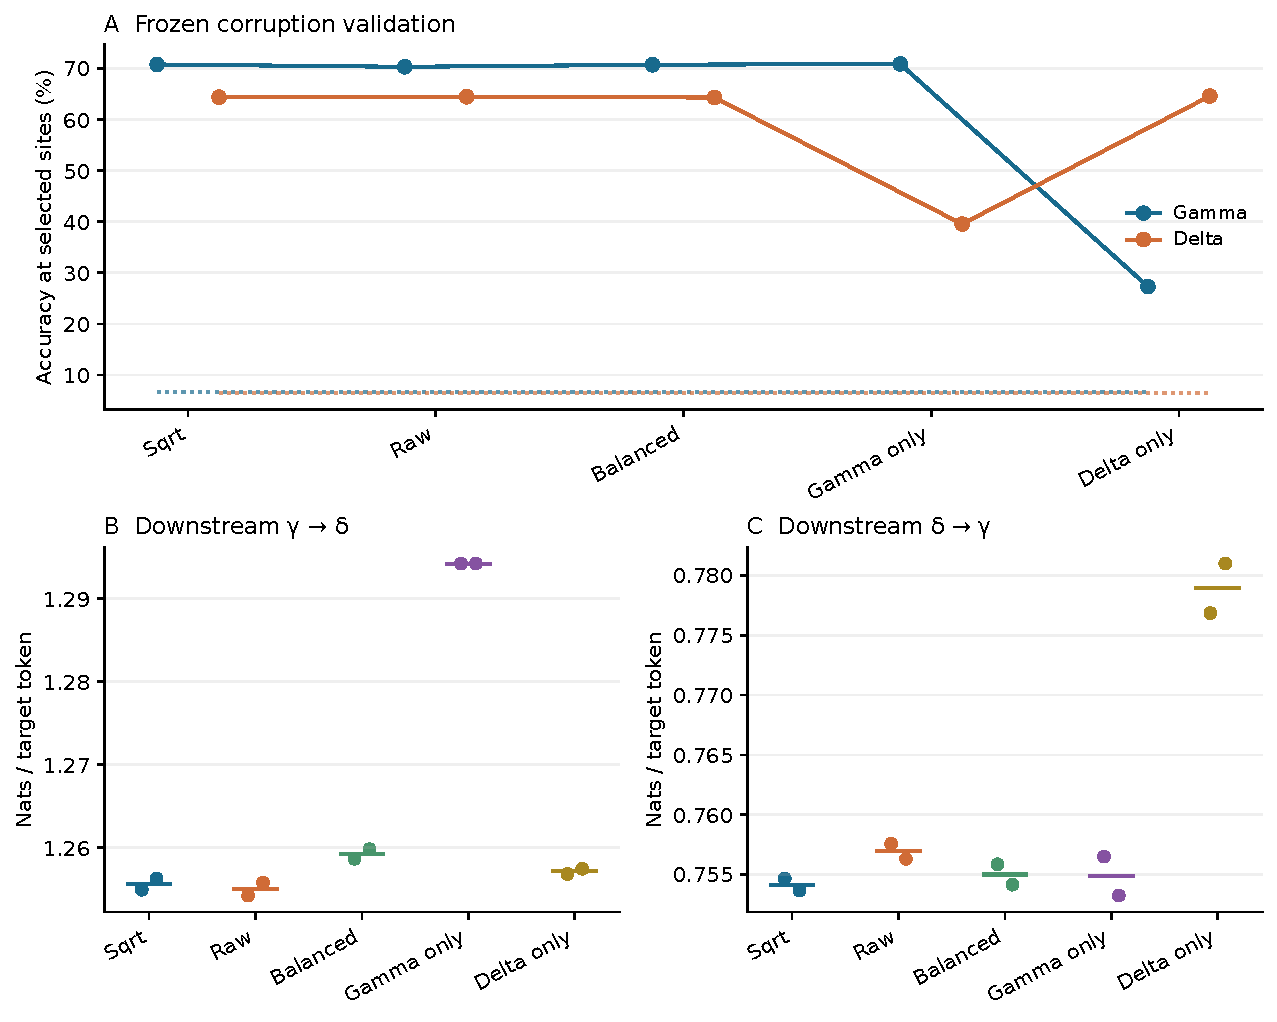
\includegraphics[width=\linewidth]{../results/bmc/figures/figure_S1_pretraining.pdf}
\caption{Pretraining mixture sensitivity. Dots retain fitted seeds. Equal sequence draws do not imply equal chain-specific or token exposure. Reconstruction is a single-chain endpoint.}
\label{fig:figure_S1_pretraining}
\end{figure}
\FloatBarrier

\subsection{Changing negative training does not resolve candidate scarcity}
Random-only and mixed negative training at ratios one, three and five reuse the
same split-17 generator candidates and retrieval pools
(Figure~\ref{fig:figure_S2_negative_training}). All twelve fitted rankers have
zero free-generation \gtd{} Hit@5. For \dtg{}, individual fitted values range
from zero to 0.22\% (zero to two of 900 queries), with no monotonic gain from
increasing the ratio. The primary mixed/3 setting averages 0.11\%; random/5,
mixed/1 and mixed/5 each average 0.17\%. Such small event differences do not
establish a reproducible recovery advantage: paired intervals for every
alternative negative setting versus the primary setting include zero in both
directions and both fitted seeds.

Fixed-pool differences are larger but depend on the comparison. In random
retrieval pools, random/3 gives two-seed mean ranker Hit@5 of 10.8\% for
\gtd{}, compared with 8.2\% under mixed/3. For \dtg{}, random/5 gives
9.1\%, compared with 7.1\% under mixed/3. These descriptive rankings are not
uniform across pools or seeds, and no setting supplies candidates absent from
the frozen free-generation set. Negative-draw and fallback counts, selected
steps and paired contrasts are retained in the numerical supplement. None of
these constructed-negative comparisons identifies biological incompatibility.


\begin{figure}[!htbp]
\centering
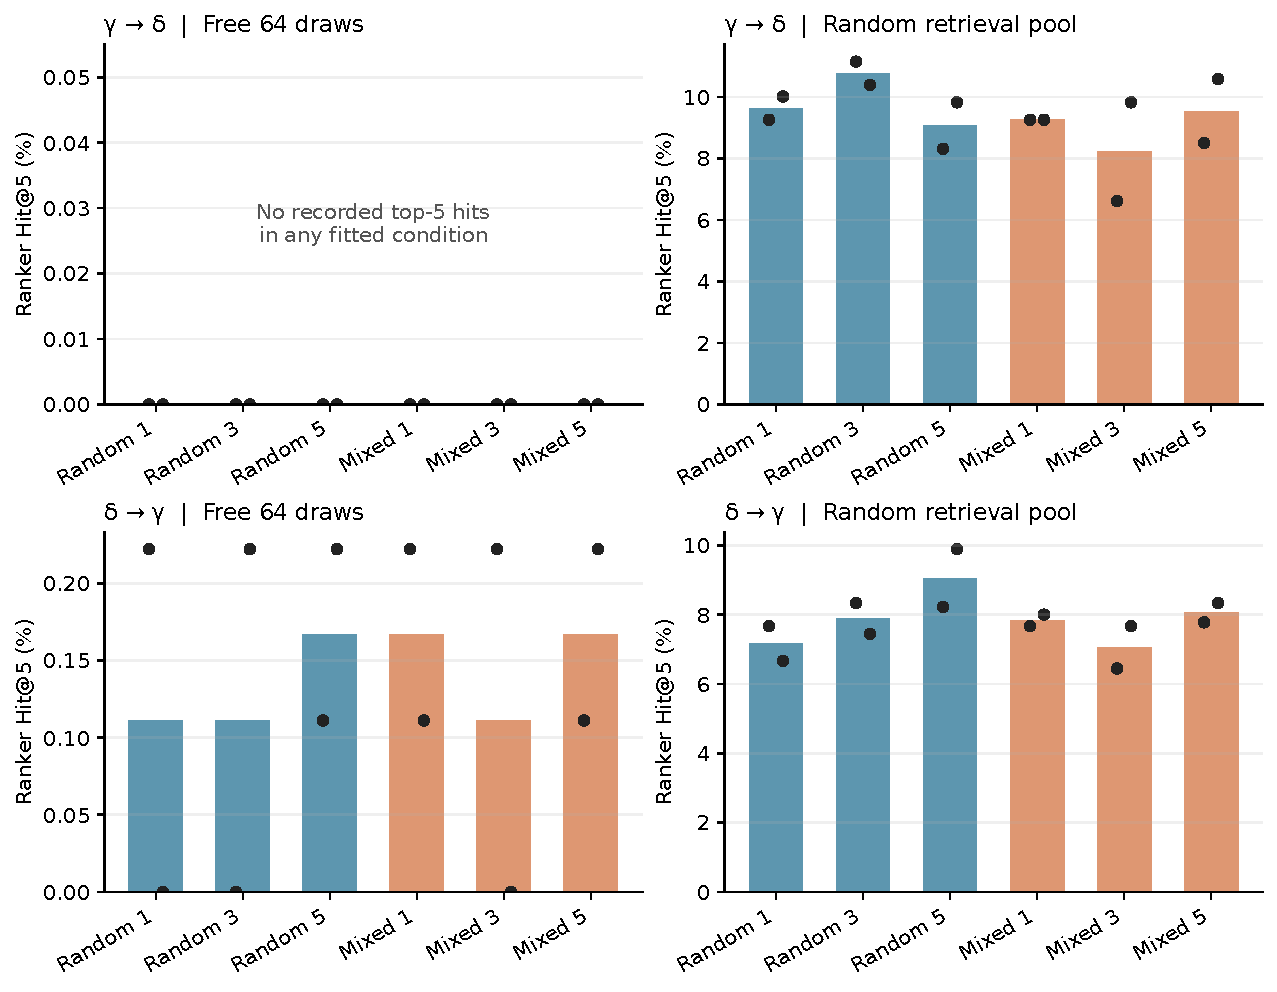
\includegraphics[width=\linewidth]{../results/bmc/figures/figure_S2_negative_training.pdf}
\caption{Ranker negative-sampling sensitivity. All settings reuse the same saved free candidates and frozen truth-containing retrieval pools. No ranker adds absent candidate sequences.}
\label{fig:figure_S2_negative_training}
\end{figure}
\FloatBarrier


\section{Nearest-input baselines and exposure diagnostics}
Nearest-input transfer uses the normalized full-CDR3 distance, lexicographic
input ties and training-degree/lexicographic target ordering. One nearest
input is primary; five is a fixed sensitivity. At most 64 unique training
targets are returned. In seen-input/withheld-edge tasks the exact input is its
own nearest neighbor, so one-neighbor transfer cannot recover its withheld
edges. Primary component-disjoint transfer is also structurally zero because
all test targets are absent from training. These zero outcomes do not identify
a learned-model mechanism. The separate nearest-input partner-similarity retrieval
score extends to the role-specific target universe using minimum target edit
distance to the nearest input's known training partners. Neither neighborhood
size nor distance rule was selected using test outcomes. Test memberships,
query-balanced selection and the giant-component edge reservation are frozen in the
revision split manifest. These are exploratory diagnostics specified after the primary analysis.

\subsection{Unseen-gamma validation design and historical estimates}
\label{sec:historical}
The original selection partition contained one gamma query with 581 recorded
partners and no ranking distractors. Its ranker selection MRR was identically
one. Original conditional likelihood Hit@5 was 9/64 in each seed (14.06\%),
compared with 9/64 and 8/64 for constant source (14.06\%/12.50\%). These
estimates are retained for traceability, not as robust unseen-gamma evidence.
The query-balanced-selection refits preserve the original train, aggregate validation
and test memberships and replace this diagnostic in the main text. Primary
component-disjoint results remain unchanged. The query-balanced selection has 31
gamma queries, 275 edges, a largest query with 137 partners and at least 118
eligible distractors per query. The tuning and calibration roles each contain
16 disjoint gamma queries and are not used for new tuning for these refits.

\subsection{Source and component-stratified descriptive analyses}
Additional file 2 includes primary source and source-distance strata and a
post-hoc source-balanced description. The latter averages nonempty source
membership strata equally. Memberships can overlap, and very small source
strata are unstable; this is neither a reweighted primary endpoint nor a
source-independent inferential comparison. Post-hoc component-size tables group
primary-test components into 1, 2--5, 6--20 and more than 20 edges, retaining
the original query positives and saved candidates. Nonempty bins give counts
and descriptive means without inferential intervals. The distant-edge recheck recovers
5, 5 and 3 primary edges, with no new claim of distant-sequence transfer.
Within-giant-component estimates originate from one original component and
deliberately have no inferential interval. Additional file 4 retains every
diagnostic query outcome, including zero events, all control conditions and
paired contrasts. Additional file 3 records actual generator sequences and
target tokens; ranker encoded-token counts were not logged and are not imputed.



\subsection{Query-balanced unseen-gamma evaluation}
The query-balanced validation has 31 selection queries with eligible distractors, and
ranker selection MRR is no longer identically one: the selected values are
0.1405 and 0.1618. Training and test memberships remain unchanged. At 64 free
draws, conditional likelihood recovers 8/64 and 10/64 queries, compared with
8/64 and 9/64 for constant source, 10/64 and 8/64 for random initialization,
and 6/64 and 7/64 for shuffled input. These counts also equal coverage for
each fitted generator. Conditional-minus-prior Hit@5 differences are 0.00
percentage points (95\% source-query interval $[0.00,0.00]$) and 1.56 points
($[0.00,4.69]$). The small number of discordant events limits inference.
Ranker ordering recovers 6/64 and 8/64 queries, two fewer than likelihood in
each seed. One-neighbor and five-neighbor direct partner transfer recover 3/64
and 7/64 queries, respectively. The repaired test still permits target
exposure: 252 distinct recorded target deltas also occur in training.
These query-balanced results supersede the original single-query-selection
diagnostic, whose estimates remain in Section~\ref{sec:historical}. They do not establish
a reproducible conditional free-recovery advantage over the matched prior.

\subsection{Within-component withheld-edge evaluation}
Within the exposed giant component, conditional coverage is 70/177 and 62/177
gamma queries and 155/261 and 164/261 delta queries. Likelihood Hit@5 is
60/177 and 50/177 for \gtd{} (33.90\%/28.25\%), and 123/261 and 118/261 for
\dtg{} (47.13\%/45.21\%; main Figure 6). Constant-source
Hit@5 is 47/177 in both gamma-query fits and 113/261 and 121/261 for delta
queries. Shuffled-input counts are 57/177 and 54/177, and 126/261 and 116/261,
respectively. Random initialization yields 32/177 and 27/177, and 121/261 and
124/261. Thus, much of the high recovery persists without the correct input
association; a conditional-minus-prior advantage is not consistent across
directions and seeds.

Ranker ordering gives 30/177 and 35/177 gamma-query hits and 71/261 and 94/261
delta-query hits, below likelihood in all four fits. Direct transfer from one
nearest input has zero hits in both directions: the nearest input is the query
itself, whose remaining training partners exclude its withheld edges. The fixed five-neighbor
sensitivity recovers 4/177 and 57/261 queries. These proposals contain copied
training partners and use a different candidate mechanism from stochastic
generation. All 500 test edges retain both endpoints in supervised training
and originate from one original graph component. The results are point
estimates and counts, without an inferential component-bootstrap interval.
Their contrast with the primary task describes different graph populations
and training composition, rather than distant or unseen-component transfer.

\FloatBarrier


\subsection{Directional exposure comparisons}
Other directional tasks also have higher recovery than the both-chain-unseen
primary task (main Figure 6). For unseen delta inputs, conditional \dtg{} Hit@5 is 39.75\%/38.51\%,
compared with 41.61\%/39.13\% for the prior. This test has 161 queries and
244 distinct recorded target gammas shared with training. Thus, substantial
recovery in a target-exposed task does not itself demonstrate an input-specific
advantage. In seen-input/unseen-edge tests, conditional Hit@5 is
6.89\%/6.67\% for \gtd{} versus 5.33\%/5.33\% for the prior, and
32.58\%/34.09\% for \dtg{} versus 30.30\%/29.92\%. These populations,
edge counts and permissible overlaps differ from the primary test and are
reported as distinct diagnostics, with source-query-group intervals.
For seen delta inputs, conditional-minus-prior Hit@5 differences are 2.27
percentage points (95\% interval $[-1.52,6.06]$) and 4.17 points
($[0.38,8.33]$). The latter fitted contrast is positive, but the two-seed
result is not uniform and does not transfer to both-chain-unseen generation.

\subsection{Study-level exposure comparisons}
Strict study holdout has 207 gamma and 419 delta queries over 626 pairs.
Conditional \dtg{} likelihood Hit@5 is 11.93\%/10.26\%, compared with
6.68\%/6.44\% for constant source and 8.83\%/9.79\% for shuffled input.
Conditional-minus-prior differences are 5.25 percentage points with a 95\%
component interval $[0.00,6.23]$ and 3.82 points with $[0.00,4.48]$;
both intervals reach zero despite positive fitted differences.
When shared supervised chains are retained, the corresponding conditional
values increase to 47.49\%/44.39\%; constant source already reaches
43.68\%/43.20\%, and shuffled input reaches 43.68\%/43.91\%.
The shared-source conditional-minus-prior differences are 3.82 percentage
points ($[-2.13,4.69]$) and 1.19 points ($[0.00,1.42]$), again with paired
component intervals including zero.
For \gtd{}, conditional likelihood Hit@5 is zero in both seeds under both
source protocols. Source results therefore cannot be reduced to uniform
failure, nor can high \dtg{} recovery be attributed entirely to conditioning.

The source test contains 90 components, with 529 of 626 edges and 323 of 419
delta queries in its largest component. A post-hoc description of the saved
query outcomes finds 50 of 50 and 42 of 43 strict-source conditional top-five
hits in that component. The corresponding shared-source counts are 198 of 199
and 184 of 186. This concentration motivates the clustered uncertainty rather
than treating all hits as independent replications. The source protocols share
the same test set and filtered pretraining pool, but supervised training contains
4956 versus 7597 edges. Shared-source training overlaps the test in 144 gamma
and 13 delta sequences. Exposure and training composition therefore change
together. Neither protocol supports a donor-independent or distant-sequence
generalization claim.

Ranker-only \dtg{} Hit@5 is 3.10\%/2.86\% under strict source holdout and
14.32\%/13.60\% under shared source, below likelihood in all four fits.
The higher source-task recovery consequently does not support a
separate-ranking benefit.


\section{Sampling budgets, decoding and calibration}
Split-17 conditional \dtg{} coverage increases from 0.67\%/0.33\% at 16
draws to 2.33\%/1.44\% at 64 and 6.33\%/6.22\% at 256 for model seeds
3407/3508. Nevertheless, with training targets allowed, likelihood Hit@5 is
0.22\%/0.11\%, 0.22\%/0.00\% and 0.00\%/0.00\%, respectively
(Figure~\ref{fig:sampling}). Additional samples can introduce high-scoring
competitors as well as recorded partners. The 256 draws average approximately
203 unique valid gamma candidates per query, but only about 53\% of raw
gamma draws differ from supervised-training targets. For \gtd{}, approximately
88\% of draws are novel and about 244 unique candidates remain at 256 draws;
coverage is 0.57\% in each seed and likelihood Hit@5 remains zero.

Excluding exact training targets changes ordering without increasing the
sampling budget. Because primary-test targets are chain-disjoint from training,
their coverage is unchanged. At 256 draws, \dtg{} likelihood Hit@5 increases
to 1.89\%/2.44\%, while \gtd{} reaches 0.57\%/0.19\%. This policy result
is reported separately from the frozen primary endpoint. It cannot be applied
unchanged as a general advantage in shared-target tasks, where exclusion may
remove a legitimate test partner.

The six-cell tuning-only temperature/top-$p$ grid has zero likelihood Hit@5
in both directions for both fitted seeds at 64 draws. The prespecified tie
rule retains temperature one and top-$p=0.95$; these sparse tuning outcomes
do not establish an improved decoding setting. All grid cells and their
coverage, validity, uniqueness and novelty are included in Additional file 4.

Free-candidate calibration contains no recorded \gtd{} positive in any
primary fit, triggering the specified reject-all rule. The \dtg{} calibration
sets contain only one to six recorded positive candidates. Their selected
likelihood/fused thresholds accept at least one candidate for every test query,
without improving the very sparse top-five hits. These calibration data do not
establish a useful operating point for biological candidate selection.

Deterministically chosen descriptive examples illustrate both failure stages.
For split 17/model seed 3407 in \dtg{}, 879 of 900 queries lack a recorded
partner in the 64-draw candidate set, 19 contain one outside the likelihood
top five, and two yield a top-five hit. In \gtd{}, the corresponding counts
are 527, two and zero out of 529 queries. Additional file 4 records the first
input in lexicographic order within each nonempty category and preserves its
positives, ranked candidates and training-target flags. These examples are
post-hoc descriptions, not additional independent validation.

\begin{figure}[!htbp]
\centering
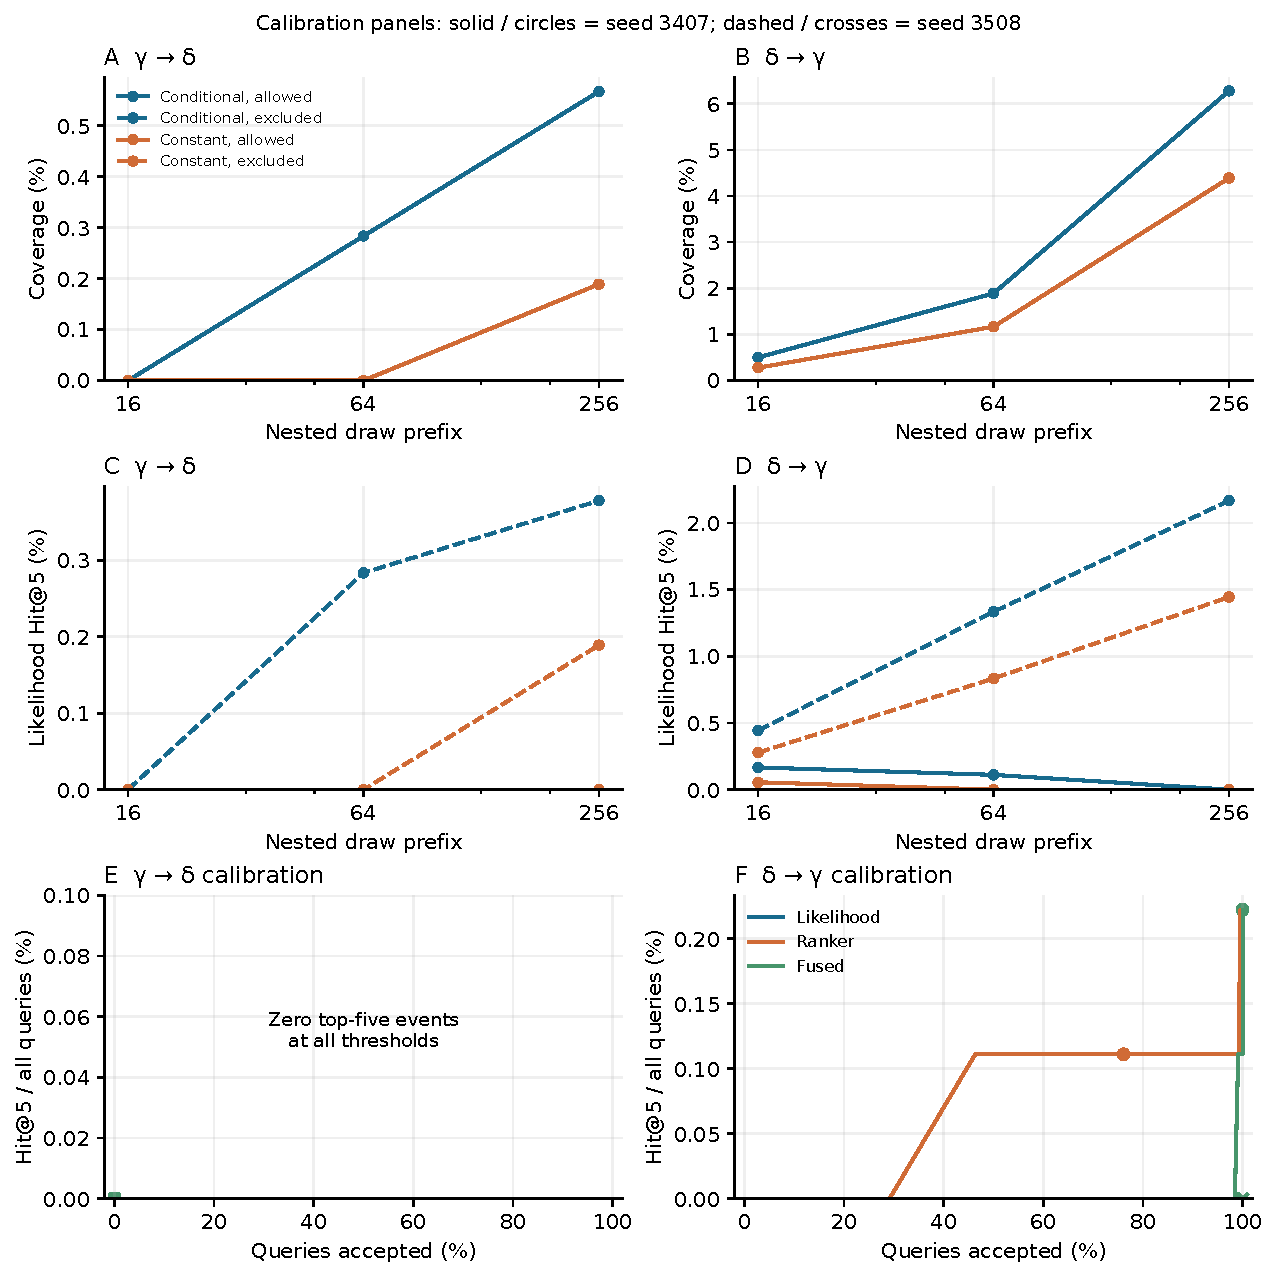
\includegraphics[width=\linewidth]{../results/bmc/figures/figure_7_budget.pdf}
\caption{Sampling budgets and exploratory calibration. The 16/64/256 budgets are prefixes of the same saved draws on split 17. The first two rows separate candidate coverage from likelihood Hit@5, with exact training targets allowed (solid) or excluded (dashed); lines average two seeds. Coverage is unchanged by target exclusion in the chain-disjoint primary test. The last row shows exploratory calibration-quantile operating curves; solid/dashed lines identify seeds and markers identify independently calibrated thresholds. All test queries remain in recovery denominators. More draws can increase coverage without improving top-five ordering. No threshold is a validated biological selector.}
\label{fig:sampling}
\end{figure}
\FloatBarrier

\end{document}
